\chapter{Marine Electric Propulsion}
\section{Introduction}
\subsection{The propulsion requirement}
At constant speeds, the thrust produced by the propeller(s) will equal the resistive force experienced by the ship as it moves through the water i.e. balancing of forces at a given speed. When propeller thrust exceeds the resistive force of the ship then it will accelerate. If resistance exceeds thrust then the ship will de-accelerate until the force equilibrium is restored.
\begin{figure}[H]
    \centering
    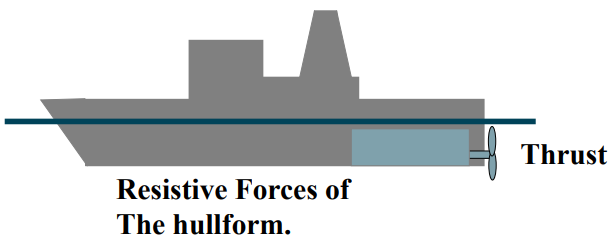
\includegraphics[width = \textwidth]{img/figure52.png}
    \caption{Ship force diagram.}
\end{figure}
\subsection{Effective power}
\textbf{\underline{Definition:}} the product of the speed of the hullform through the water and its resistance at that speed.

\textbf{\underline{Equation:}}
\begin{gather}
    \textrm{Effective power}=R_T\cdot V_s \, \si{\kilo\watt}
\end{gather}

\textbf{\underline{Simple example:}} at \SI{3}{\meter\per\second} the effective tow rope pull of a naked hull is \SI{50}{\kilo\newton}. Find the power of the hull at this speed.
\begin{gather}
    P_E = 50\times 3=\SI{150}{\kilo\watt}
\end{gather}
\subsection{The generalised resistance equation}
The generalised resistance equation is:
\begin{gather}
    R_{total} = R_{frictional} + R_{form} + R_{wave} + R_{air}
\end{gather}
At low speeds $R_{frictional}$ tends to dominate $R_{total}$. At high speeds $R_{wave}$ tends to dominate $R_{total}$. `Rule of thumb' - it is acceptable to assume the resistance of a ship is proportional to the square of the ship speed ($V_{ship}$). For monohulls:
\begin{gather}\label{8.e2}
    R_{total} = C_1 \cdot V_{ship}^2
\end{gather}
\subsection{Propulsive power requirement}
Effective power $P_E$ is \underline{not} the same as shaft power. As a first approximation $P_E$ may be determined from:
\begin{gather}\label{8.e3}
    P_E = R_{total} \cdot V_{ship}
\end{gather}
Combining \eqref{8.e2} and \eqref{8.e3}, we have:
\begin{gather}
    P_E = C_1 \cdot V_{ship}^3
\end{gather}
where, $C_1$ is not a constant but contains a factor $C_0$ that is speed dependent and a multiplying factor $y$, which depends upon ship operational characteristics and in particular degradation of performance.
\subsection{Relationship between speed and power}
This means that if the ship's speed is doubled then the power required to achieve that speed is increased eight fold. This also means fuel consumption could also increase by a similar factor.
\begin{gather}\label{8.e5}
    C_1 = y \cdot C_0 V_{ship}\\
    y = \textrm{function/fouling, displacement, sea-state, water-depth}
\end{gather}
Losses incurred by the propulsors mean a higher shaft power is required from the engines. Typically, FPP (fixed pitch propeller) efficiency is 70-75\% but values are different at different speeds and actual values depend upon propulsor design characteristics such as pitch, diameter, rotational speeds and also upon operational conditions such as depth of propeller in the water and wake characteristics. $\eta_{propeller}$ is therefore speed dependent.
\subsection{Shaft power and effective power}
The required shaft power, $P_s$, is calculated from:
\begin{gather}
    P_s = P_E + \textrm{propulsor lost power} = \underline{P}_e (\eta_{propeller})
\end{gather}
The shaft power, $P_s$, is supplied by the propulsion machinery to the propulsion shaft and is calculated from:
\begin{gather}
    P_s = \omega \cdot T_s\\
    \omega = 2\pi N_s
\end{gather}
where $T_s$ is shaft torque and $N_s$ is shaft revolutions per second. There are limitations on the maximum rotational speed of the propulsor hence torques can be large!
\subsection{Ship power/speed curves}
\begin{figure}[H]
    \centering
    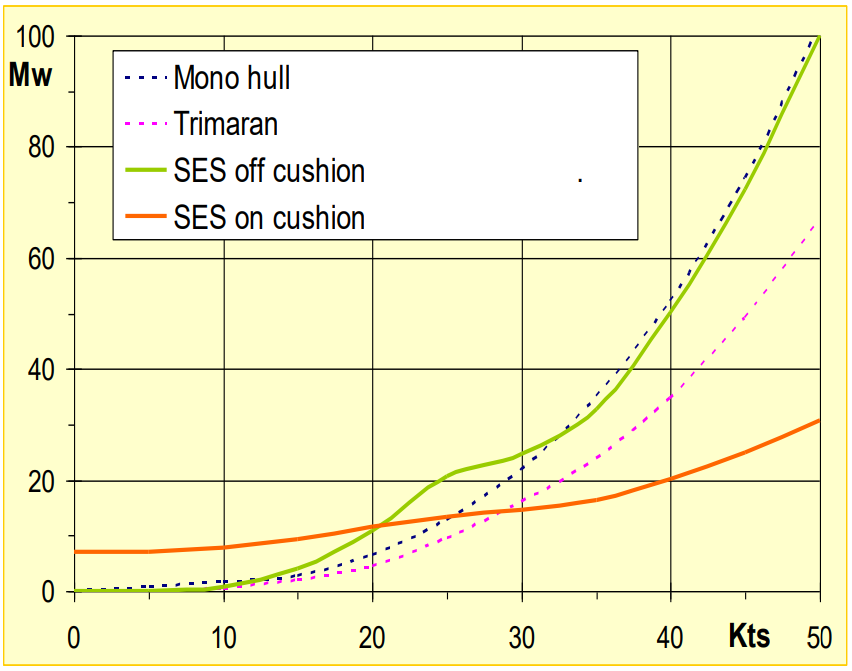
\includegraphics[width =0.8 \textwidth]{img/figure53.png}
    \caption{Ship power/speed curve.}
\end{figure}
This relationship is acceptable for relatively low speeds but at high speeds the resistance will tend to increase at increasing rates with increases in ship's speed. Note: the difference between the curves for monohull and multi-hull vessels for this fast corvette example.
\subsection{Power speed/curve - two shafts}
\begin{figure}[H]
    \centering
    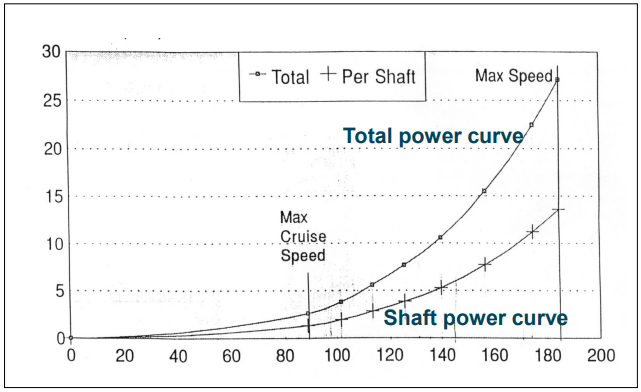
\includegraphics[width =0.8 \textwidth]{img/figure54.png}
    \caption{Power speed/curve - two shafts.}
\end{figure}
Twin shaft naval frigate with maximum speed of \SI{29}{knots} (\SI{185}{rpm}) and cruising speed of \SI{14}{knots} (\SI{90}{rpm}).
\subsection{Main components of a marine propulsions system}
The propulsion system is one of the key `systems' in any ship or submarine. The function of any propulsion system is to generate thrust to move the ship at some desired speed in some direction. The main components of a propulsion system are:
\begin{itemize}
    \item The Prime-mover(s)
    \item The Transmission system(s)
    \item The Propulsor(s)
\end{itemize}
\subsection{Efficiency of electrical propulsion}
\begin{figure}[H]
    \centering
    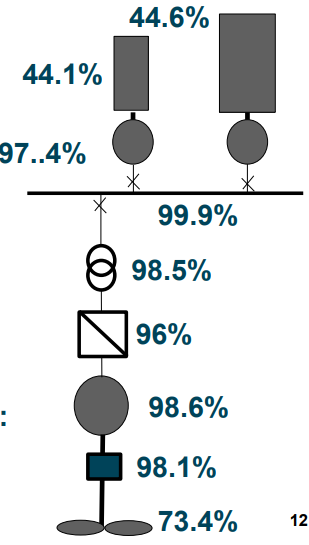
\includegraphics[height = 7cm]{img/figure55.png}
    \caption{Ship SLD efficiency.}
\end{figure}
\begin{table}[H]
    \centering
    \begin{tabular}{@{}ll@{}}
        \toprule
        \textbf{Item}   & \textbf{Efficiency} \\
        \midrule
        Diesel Engine 1 & 44.6\%              \\
        Diesel Engine 2 & 44.1\%              \\
        Generator       & 97.4\%              \\
        Transmission    & 99.9\%              \\
        Transformer     & 98.5\%              \\
        Converter       & 96\%                \\
        Motor
                        & 98.6\%              \\
        Gearbox         & 98.1\%              \\
        Propeller       & 73.4\%              \\
        \bottomrule
    \end{tabular}
    \caption{Example efficiencies of components in a marine propulsion system.}
    \label{8.t1}
\end{table}
`Overall propulsion' efficiency can be defined as:
\begin{gather}
    \eta = \frac{\textrm{Energy available for useful thrust}}{\textrm{Calorific energy available in fuel}}
\end{gather}
Efficiency of system defined in Table \ref{8.t1}: 28.97\% (at normal speed).
\section{Marine electric propulsion}
\subsection{The early days}
\begin{itemize}
    \item The pioneers
    \item Battery powered propulsion
    \item Turbo-electric (AC) propulsion
    \item Diesel-electric (DC) propulsion
    \item Reasons for the decline of conventional electric propulsion systems
\end{itemize}

\begin{figure}[H]
    \centering
    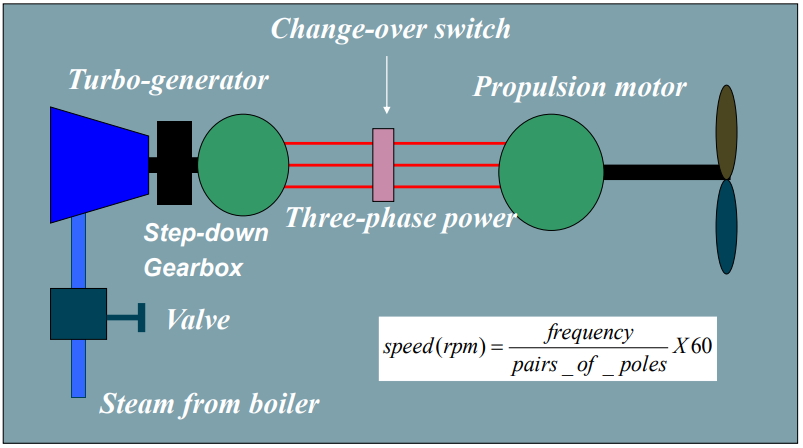
\includegraphics[width = 0.8\textwidth]{img/figure56.png}
    \caption{Turbo-electric propulsion (Emmet) system.}
\end{figure}
An `electrical speed reduction gearbox' simply facilitated by the step-up ratio of generator to motor poles.

\textbf{Features of the turbo-electric propulsion:}
\begin{itemize}
    \item Avoided the need for a complex gearbox to reduce revolutions between a high speed turbine and a low speed propeller shaft
    \item Avoided the need for stringent alignment of the propulsion system within the ship thus allowing greater flexibility in layout especially in large ships
    \item Enabled simple reversing by ise of change-over switch rather than a separate reversing turbine
    \item It is perceived that more conversion stages meant more equipment in the shaft line hence greater losses (especially at high ship speeds) therefore greater through life cost
\end{itemize}

\begin{figure}[H]
    \centering
    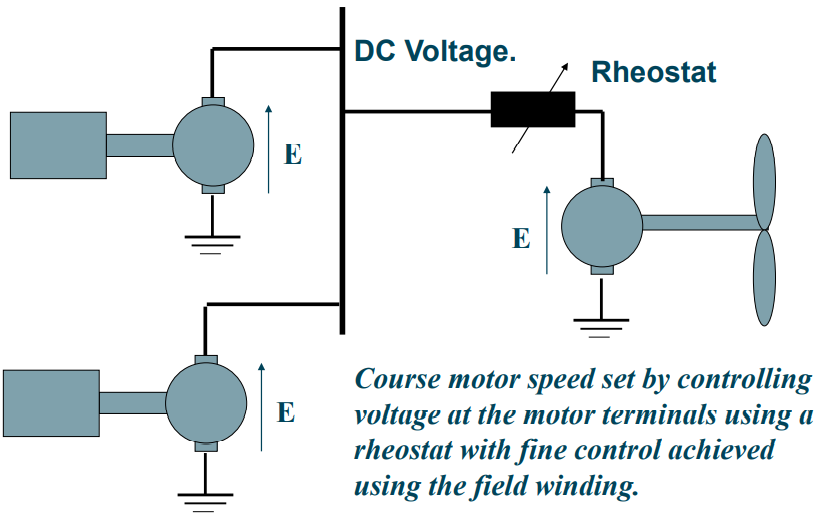
\includegraphics[width = 0.8\textwidth]{img/figure57.png}
    \caption{Diesel-electric (DC) propulsion system.}
\end{figure}

\textbf{Decline of the conventional propulsion systems:}
\begin{itemize}
    \item Cost of oil increased leading to the demand for more efficient propulsion systems (e.g. 1970's oil crisis)
    \item Growth of offshore exploration for oil and gas led to the demand for greater controllability of propulsion power including dynamic positioning control (e.g. North Sea and Gulf of Mexico)
    \item The demand for AC distribution systems for ship's services and to integrate with propulsion power (i.e. DC was considered old fashioned)
    \item The invention of power electronic devices (especially the thyristor) and the introduction of power electronic converters
\end{itemize}

\subsection{Modern ship designs}
\begin{itemize}
    \item The modern diesel-electric DC propulsion system
    \item The constant speed propulsion motor system
    \item The re-engineering of the QEII
\end{itemize}

\begin{figure}[H]
    \centering
    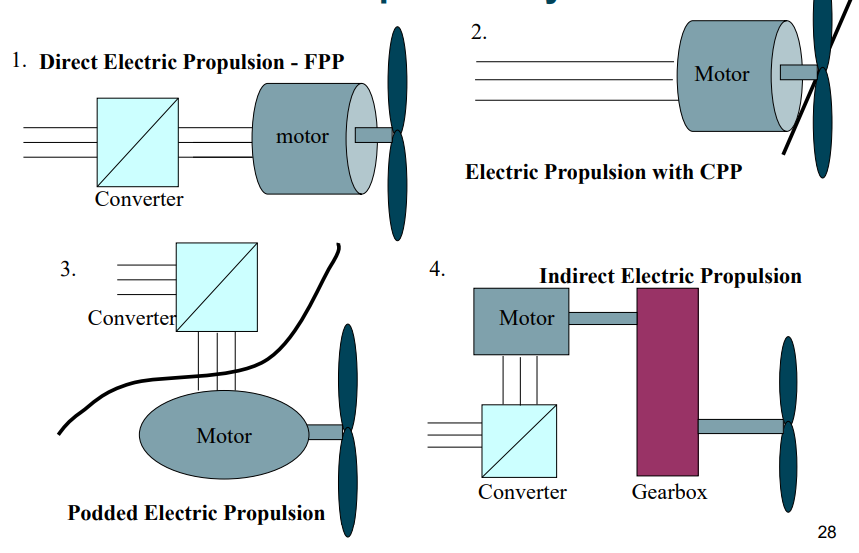
\includegraphics[width = 0.8\textwidth]{img/figure58.png}
    \caption{Modern electric propulsion systems.}
\end{figure}
FPP - fixed pitch propeller, CPP - controllable pitch

\begin{figure}[H]
    \centering
    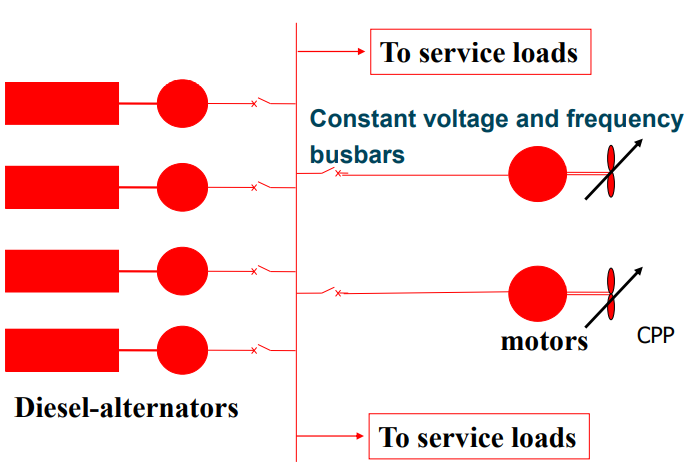
\includegraphics[width = 0.8\textwidth]{img/figure59.png}
    \caption{Electrical propulsion with CPPs.}
\end{figure}

\begin{figure}[H]
    \centering
    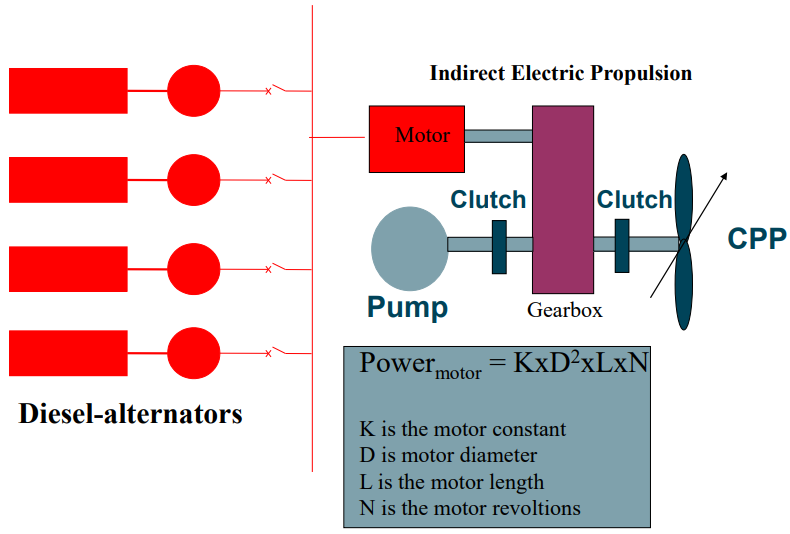
\includegraphics[width = 0.8\textwidth]{img/figure60.png}
    \caption{Electrical propulsion with gearboxes.}
\end{figure}

\begin{figure}[H]
    \centering
    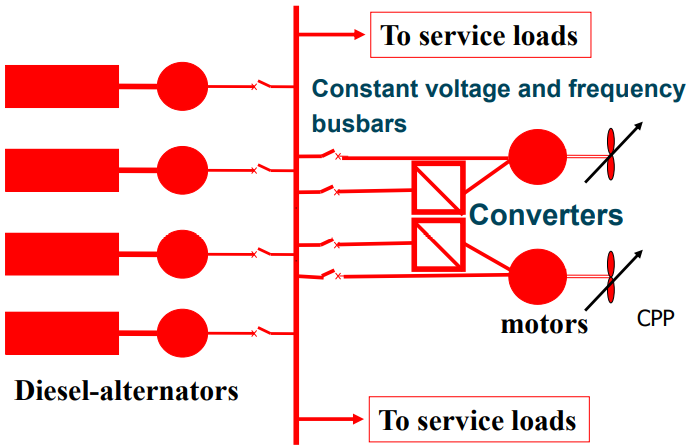
\includegraphics[width = 0.8\textwidth]{img/figure61.png}
    \caption{Electrical propulsion with converters and CPPs.}
\end{figure}

\begin{figure}[H]
    \centering
    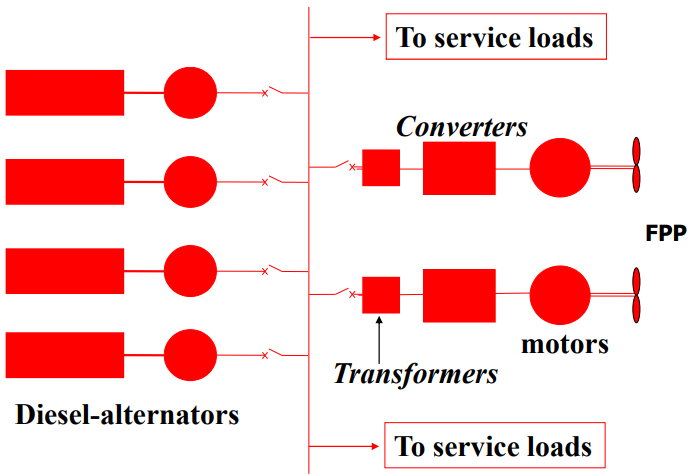
\includegraphics[width = 0.8\textwidth]{img/figure62.png}
    \caption{Electrical propulsion with converters.}
\end{figure}

\begin{figure}[H]
    \centering
    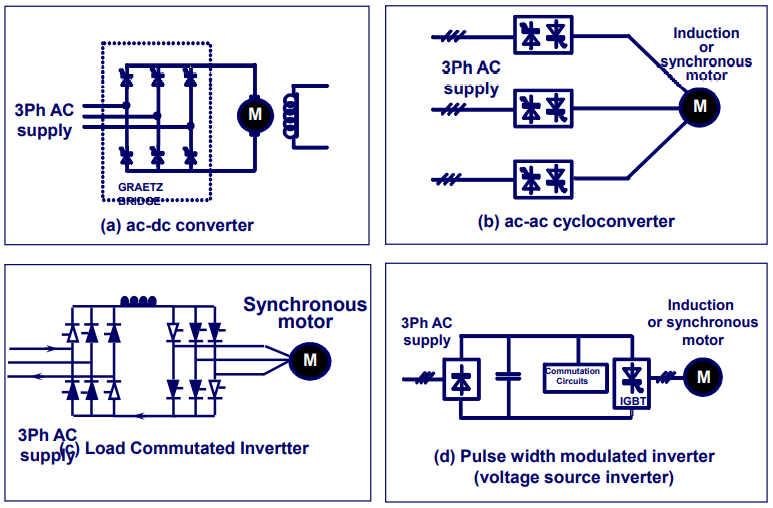
\includegraphics[width = 0.8\textwidth]{img/figure63.png}
    \caption{Main types of converters.}
\end{figure}

\textbf{Modern power converters:}
\begin{itemize}
    \item DC rectifier with DC motor
          \begin{itemize}
              \item Limited to \SI{10}{\mega\watt} at \SI{200}{rpm}
              \item Old technology now replaced with AC drives
          \end{itemize}
    \item Cycloconverter drive with AC motor
          \begin{itemize}
              \item Unlimited power
              \item Synchronous or Induction motors
              \item Transformers required
              \item Large size
          \end{itemize}
    \item Load commutator inverter with AC motor
          \begin{itemize}
              \item Unlimited power
              \item Synchronous motors only
              \item Transformers required
              \item Compact size
              \item Waveform distortion
          \end{itemize}
    \item Pulse width modulated drive with AC motor
          \begin{itemize}
              \item Power limited to \SI{24}{\mega\watt} approximately
              \item Synchronous or Induction motors
              \item Good waveform quality
              \item Developing technology
          \end{itemize}
\end{itemize}

\begin{figure}[H]
    \centering
    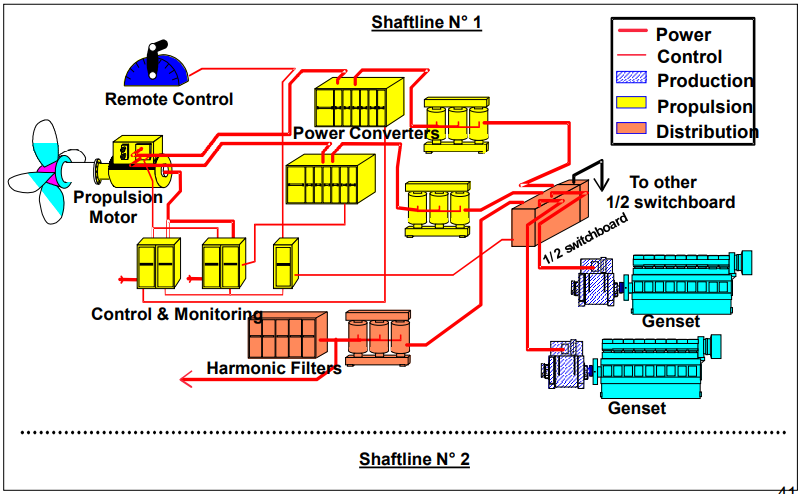
\includegraphics[width = 0.8\textwidth]{img/figure64.png}
    \caption{Electrical propulsion system arrangement.}
\end{figure}

\begin{figure}[H]
    \centering
    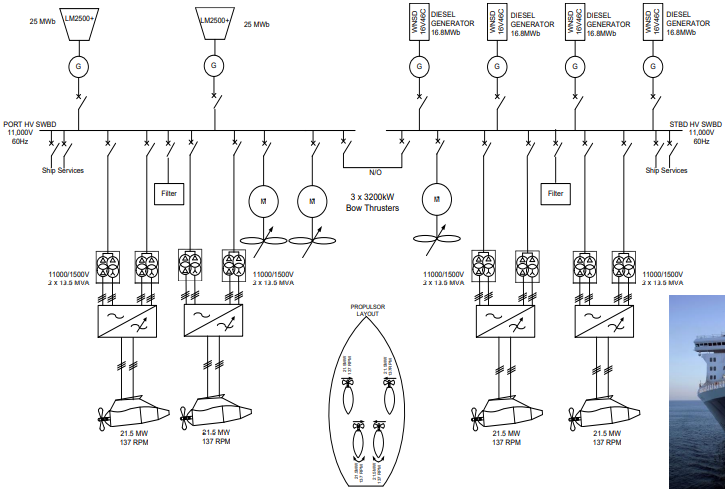
\includegraphics[width = 0.8\textwidth]{img/figure65.png}
    \caption{Queen Elizabeth 2 electrical propulsion system arrangement.}
\end{figure}

\begin{figure}[H]
    \centering
    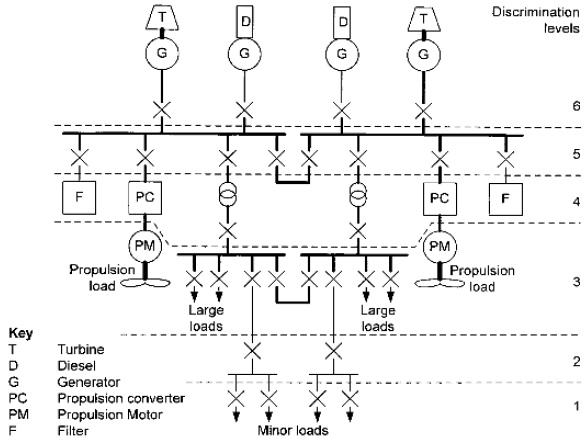
\includegraphics[width = 0.8\textwidth]{img/figure66.png}
    \caption{T45 Frigate electrical line diagram (not exact).}
\end{figure}

\begin{figure}[H]
    \centering
    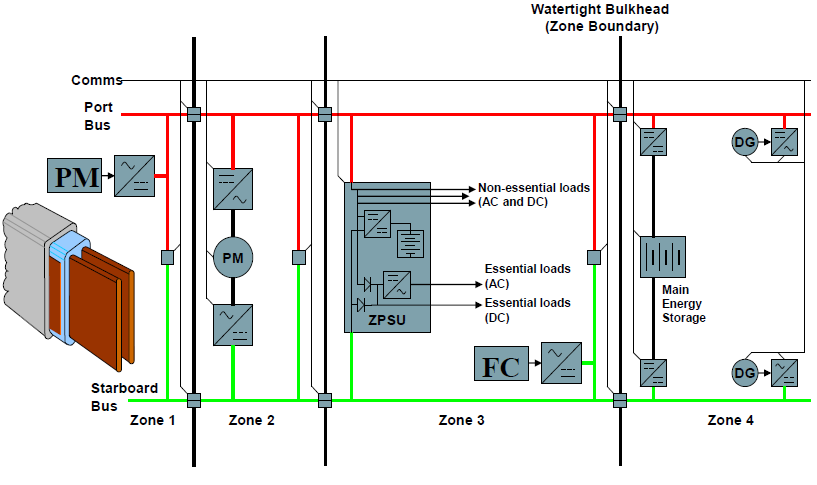
\includegraphics[width = 0.8\textwidth]{img/figure67.png}
    \caption{Zonal power example architecture.}
\end{figure}

\begin{figure}[H]
    \centering
    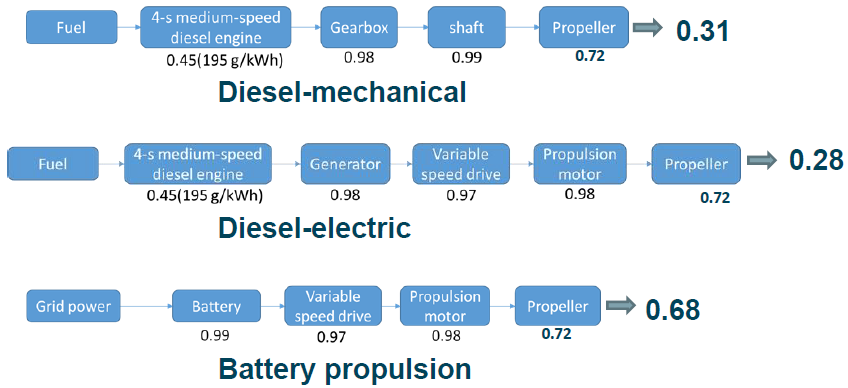
\includegraphics[width = 0.8\textwidth]{img/figure68.png}
    \caption{System configuration efficiencies.}
\end{figure}

\begin{figure}[H]
    \centering
    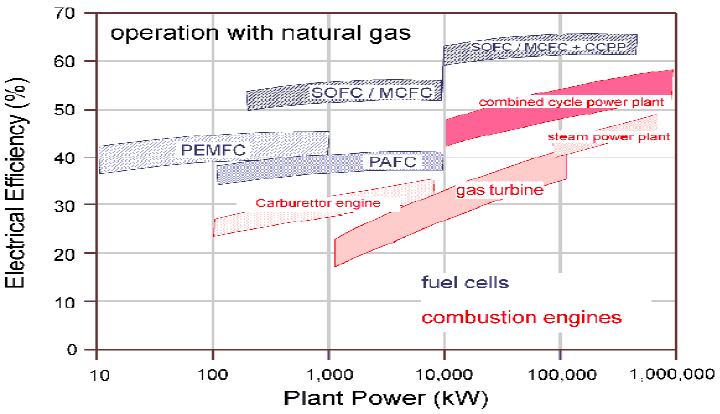
\includegraphics[width = 0.8\textwidth]{img/figure69.png}
    \caption{Potential of fuel cell technology.}
\end{figure}

\begin{table}[H]
    \centering
    \begin{tabular}{@{}llll@{}}
        \toprule
        \textbf{Power system} & \textbf{Efficiency} & \textbf{Weight power density}   & \textbf{Volume power density}     \\
                              &                     & [\si{\kilo\gram\per\kilo\watt}] & [\si{\meter\cubed\per\kilo\watt}] \\
        \midrule
        PEFC                  & 39-42\%             & 2.7-5.4                         & 0.005-0.009                       \\
        SOFC                  & 45-60\%             & 9.1-13.6                        & 0.017-0.034                       \\
        MCFC                  & 40-55\%             & 18.1-27.2                       & 0.028-0.060                       \\
        PAFC                  & 38-42\%             & 13.6-20.9                       & 0.026-0.043                       \\
        Diesel generator      & 31\%                & 14.2                            & 0.024                             \\
        Gas turbine generator & 26\%                & 12.2                            & 0.026                             \\
        \bottomrule
    \end{tabular}
    \caption{Current fuel cell technology.}
\end{table}

\textbf{Perceived advantages of modern electric propulsion:}
\begin{itemize}
    \item Can be more fuel efficient
    \item Can reduce emissions
    \item Lower maintenance saving
    \item Flexibility of operation
    \item Flexibility of design
    \item Greater redundancy
    \item Lower noise
    \item Easily reversible and good manoeuvrability
\end{itemize}

\textbf{Perceived disadvantages of modern electric propulsion:}
\begin{itemize}
    \item Greater initial cost of machinery
    \item Greater machinery volume taken up in hull
    \item Greater weight of machinery
    \item Poor efficiency at full speed
\end{itemize}

\subsection{Summary}
\begin{itemize}
    \item Electrical propulsion has been used in ships for over a century. It was first established in small boats and submarines
    \item Modern electrical propulsion systems are extensive in design but are largely based upon the use of power conversion methods
    \item The purpose of power conversion is to convert a fixed voltage/fixed frequency supply to a variable voltage and variable frequency for the control of the propulsion motor speed
    \item Electrical propulsion is firmly established in UK naval ships and is being seriously considered for use in future US naval vessels and other naval ships across the world. It is already used extensively in merchant ships of all kind
    \item Electric propulsion technology continues to develop with new equipment and systems designs
\end{itemize}